\chapter{Evaluierung}
\label{chap:eval}
\todo[size=\small, color=blue!40, inline]{Kapitel: Evaluierung}%
\begin{itemize}
 \item wie skaliert das System / bringt es was?
 \item Balancierung durch $c$-Collision Protokoll / die Varianz
 \item Netzwerk ist wichtig $\rightarrow$ hat sich in den tests gezeigt. Siehe MiniCluster.
\end{itemize}
\todo[size=\small, inline]{Diagramme für Reload: eins mit median und 10\% Quantilen aus einem durchgang; evtl. gemittelt; eins mit min-, oder max-, oder median-werten}%
\todo[size=\small, inline]{absolutes in und max bei den Quantilen angeben und dann einen Block für die Quartile (0.25 und 0.75) und dann den Median eintragen.}%

Um die Effektivität des in dieser Arbeit entstandenen Systems überprüfen zu können, wurden verschiedene Tests durchgeführt.
Beim ersten Test, dem \textit{FPS-Test}, wurden bei einem Walkthrough durch die Szene die Bilder pro Sekunde aufgezeichnet. Der \textit{Reload-Test} hat bei verschiedenen Systemkonfigurationen an festen Kamerapositionen die Zeit gemessen, die ein erneutes Laden der Szene benötigt. Beim \textit{$c$-Collision-Test} wurde die List auf den einzelnen Datenknoten gemessen. Die einzelnen Testläufe unterscheiden sich dabei in der verwendeten Anzahl an Datenknoten und Redundanzen. Redundanz bedeutet, wie oft das Modell der Boeing vollständig im Netzwerk verteilt wurde. \\
Weitere Diagramme und Abbildungen sind in den Anhängen \ref{chap:add_diag} und \ref{chap:add_fig} zu finden.

\section{FPS-Test}
\label{sec:eval:fps}

\todo[inline]{FPS-Test - da muss ich noch mal ran!}
Bei diesem Test wurde in einem festgelegten Walkthrough durch die 3D-Szene gemessen, wieviele Bilder pro Sekunde an welcher Stelle der Szene erreicht werden konnten. Dazu wurde der Walkthrough auf je 24, 28 und 32 Datenknoten mit einer Redundanz von 1, 2 und 3 durchgeführt. Die y-Achse der Diagramme \ref{fig:eval:fps1} und \ref{fig:eval:fps3} stellt die Bilder pro Sekunde und die x-Achse die Position des Walkthroughs dar.
\begin{figure}
\centering
%%%%%%%%%%%%%%%%%%%%%%%%%%%%%%%%%%%%%%%%%%%%%%%%%%%%%%%%%
% Beispieldiagramm mit pgfplot und datenfile
%%%%%%%%%%%%%%%%%%%%%%%%%%%%%%%%%%%%%%%%%%%%%%%%%%%%%%%%%

\begin{tikzpicture}
  \begin{axis}[xlabel=Position, ylabel={FPS}, ymax=60, legend pos=north west]
    \addplot[smooth,red,samples=500] table[col sep=comma,x index=0,y index=1,header=false] {data/FPSWalkthroughTest_Redundance1_R2_D24.2010-1-25.log};
    \addlegendentry{24 Datenknoten}
    \addplot[smooth,green,samples=500] table[col sep=comma,x index=0,y index=1,header=false] {data/FPSWalkthroughTest_Redundance1_R2_D28.2010-1-25.log};
    \addlegendentry{28 Datenknoten}
    \addplot[smooth,blue,samples=500] table[col sep=comma,x index=0,y index=1,header=false] {data/FPSWalkthroughTest_Redundance1_R2_D32.2010-1-25.log};
    \addlegendentry{32 Datenknoten}
  \end{axis}
\end{tikzpicture}

  \caption{\label{fig:eval:fps1}FPS in einem Walkthrough. (Redundanz$=$1, 2 Renderer und 24-32 Datenknoten)}
\end{figure}
An den Diagrammen kann man sehen, dass sich die Bildrate bei verschiedenen Konfigurationen ähnelt. Allerdings lassen sich keine Zusammenhänge zwischen Bildrate und Redundanz oder Knotenanzahl herstellen. Die Bildrate gibt eher Rückschlüsse darauf, wie die Szene an den einzelnen Positionen beschaffen ist. An Stellen des Modells, wo sehr viel Geometrie angefordert werden muss, ist die Bildrate vermutlich geringer, als an Stellen, an denen weniger Angefordert wird. Hinzu kommt der Umstand, dass die Grafikkarten der Datenknoten im hier verwendeten Test-Cluster, etwas älter sind. In Testumgebungen mit aktuellerer Grafikhardware würde die Zahl der Redundanzen und der Knoten möglicherweise stärker ins Gewicht fallen.

\begin{figure}
\centering
%%%%%%%%%%%%%%%%%%%%%%%%%%%%%%%%%%%%%%%%%%%%%%%%%%%%%%%%%
% Beispieldiagramm mit pgfplot und datenfile
%%%%%%%%%%%%%%%%%%%%%%%%%%%%%%%%%%%%%%%%%%%%%%%%%%%%%%%%%

\begin{tikzpicture}
  \begin{axis}[xlabel=Position, ylabel={FPS}, ymax=60, legend pos=north west]
    \addplot[smooth,red,samples=500] table[col sep=comma,x index=0,y index=1,header=false] {data/FPSWalkthroughTest_Redundance3_R2_D24.2010-1-25.log};
    \addlegendentry{24 Datenknoten}
    \addplot[smooth,green,samples=500] table[col sep=comma,x index=0,y index=1,header=false] {data/FPSWalkthroughTest_Redundance3_R2_D28.2010-1-25.log};
    \addlegendentry{28 Datenknoten}
    \addplot[smooth,blue,samples=500] table[col sep=comma,x index=0,y index=1,header=false] {data/FPSWalkthroughTest_Redundance3_R2_D32.2010-1-25.log};
    \addlegendentry{32 Datenknoten}
  \end{axis}
\end{tikzpicture}

  \caption{\label{fig:eval:fps3}FPS in einem Walkthrough. (Redundanz$=$3, 2 Renderer und 24-32 Datenknoten)}
\end{figure}

\section{Reload-Test}
\label{sec:eval:reload}

Beim Reload-Test wurde gemessen, wie lange die einzelnen Datenknoten benötigen, bei festgelegten Kamerapositionen die Szene komplett zu laden. Dazu wurden sämtliche auf den Renderern befindliche Objekte verworfen und erneut angefordert. Wenn ein Datenknoten mit der kompletten Arbeit fertig war, hat er sich beim Masterknoten gemeldet, welcher die Zeit gespeichert hat.\\
Die Diagramme \ref{fig:eval:reload1} und \ref{fig:eval:reload2} enthalten auf der x-Achse die Kameraposition und auf der y-Achse die Render-Zeit in Sekunden. In den Diagrammen ist zu erkennen, dass der Median meist nahe am Durchschnitt liegt. Die Messungen wurden dabei mehrfach durchgeführt und die Ergebnisse wurden gemittelt. Ab und zu sind zwar einige Ausreißer zu erkennen, aber selbst die 0.25 und 0.75 Quantile liegen meist sehr dicht am Median. Das bedeutet, dass das System gut balanciert. Nur wenige Knoten benötigen mehr Zeit für die Szene als der Median. Jedoch lässt auch dieser Test keinen Zusammenhang zwischen Redundanzen, Knotenanzahl und der benötigten Zeit erkennen. Die Zeit, die eine Kamerposition zum Laden benötigt, scheint ausschlaggebend für die gesamte benötigte Zeit zu sein.

\begin{Bild}
%%%%%%%%%%%%%%%%%%%%%%%%%%%%%%%%%%%%%%%%%%%%%%%%%%%%%%%%%
% Beispieldiagramm mit pgfplot und datenfile
%%%%%%%%%%%%%%%%%%%%%%%%%%%%%%%%%%%%%%%%%%%%%%%%%%%%%%%%%

\begin{tikzpicture}
  \begin{axis}[xlabel=Kameraposition, 
	       ylabel={Zeit (Sekunden)},xtick=\empty, legend pos=north west, ymax=35]
  \addplot[color=red,
	   mark=|,dashed,
	   only marks,
	   error bars/.cd,
	   y dir=both,
	   y explicit,
	   error bar style={red, error bars options={line width=2pt}}]
    table[col sep=comma,x index=0,y index=2,y error index=3, header=false]
    {data/ReloadTest_Redundance1_R2_D24.2010-1-27.log_abs.data};
  \addlegendentry{Extrema}
  \addplot[color=cyan,
	   mark=|,
	   only marks,
	   error bars/.cd,
	   y dir=both,
	   y explicit,
	   error bar style={cyan, very thick},
	   ultra thick] 
    table[col sep=comma,x index=0,y index=4,y error index=5, header=false]
    {data/ReloadTest_Redundance1_R2_D24.2010-1-27.log_abs.data};
  \addlegendentry{Quartile}
%\begin{comment}
  \addplot[color=green,
	   only marks,
	   mark=*] 
    table[col sep=comma,x index=0,y index=6, header=false]
    {data/ReloadTest_Redundance1_R2_D24.2010-1-27.log_abs.data};
  \addlegendentry{Average}
%\end{comment}
  \addplot[color=black,
	   mark=x,
	   only marks] 
    table[col sep=comma,x index=0,y index=1, header=false]
    {data/ReloadTest_Redundance1_R2_D24.2010-1-27.log_abs.data};
  \addlegendentry{Median}
  \end{axis}
\end{tikzpicture}
  \captionof{figure}{\label{fig:eval:reload1}Reloadtest: Redundanz 1, 2 Renderknoten, 24 Datenknoten.}
\end{Bild}

\begin{Bild}
%%%%%%%%%%%%%%%%%%%%%%%%%%%%%%%%%%%%%%%%%%%%%%%%%%%%%%%%%
% Beispieldiagramm mit pgfplot und datenfile
%%%%%%%%%%%%%%%%%%%%%%%%%%%%%%%%%%%%%%%%%%%%%%%%%%%%%%%%%

\begin{tikzpicture}
  \begin{axis}[xlabel=Kameraposition, 
	       ylabel={Zeit (Sekunden)},xtick=\empty, legend pos=north west, ymax=35]
  \addplot[color=red,
	   mark=|,dashed,
	   only marks,
	   error bars/.cd,
	   y dir=both,
	   y explicit,
	   error bar style={red, error bars options={line width=2pt}}]
    table[col sep=comma,x index=0,y index=2,y error index=3, header=false]
    {data/ReloadTest_Redundance1_R2_D28.2010-1-27.log_abs.data};
  \addlegendentry{Extrema}
  \addplot[color=cyan,
	   mark=|,
	   only marks,
	   error bars/.cd,
	   y dir=both,
	   y explicit,
	   error bar style={cyan, very thick},
	   ultra thick] 
    table[col sep=comma,x index=0,y index=4,y error index=5, header=false]
    {data/ReloadTest_Redundance1_R2_D28.2010-1-27.log_abs.data};
  \addlegendentry{Quartile}
%\begin{comment}
  \addplot[color=green,
	   only marks,
	   mark=*] 
    table[col sep=comma,x index=0,y index=6, header=false]
    {data/ReloadTest_Redundance1_R2_D28.2010-1-27.log_abs.data};
  \addlegendentry{Average}
%\end{comment}
  \addplot[color=black,
	   mark=x,
	   only marks] 
    table[col sep=comma,x index=0,y index=1, header=false]
    {data/ReloadTest_Redundance1_R2_D28.2010-1-27.log_abs.data};
  \addlegendentry{Median}
  \end{axis}
\end{tikzpicture}
  \captionof{figure}{\label{fig:eval:reload2}Reloadtest: Redundanz 1, 2 Renderknoten, 28 Datenknoten.}
\end{Bild}
\begin{Bild}
%%%%%%%%%%%%%%%%%%%%%%%%%%%%%%%%%%%%%%%%%%%%%%%%%%%%%%%%%
% Beispieldiagramm mit pgfplot und datenfile
%%%%%%%%%%%%%%%%%%%%%%%%%%%%%%%%%%%%%%%%%%%%%%%%%%%%%%%%%

\begin{tikzpicture}
  \begin{axis}[xlabel=Kameraposition, 
	       ylabel={Zeit (Sekunden)},xtick=\empty, legend pos=north west, ymax=35]
  \addplot[color=red,
	   mark=|,dashed,
	   only marks,
	   error bars/.cd,
	   y dir=both,
	   y explicit,
	   error bar style={red, error bars options={line width=2pt}}]
    table[col sep=comma,x index=0,y index=2,y error index=3, header=false]
    {data/ReloadTest_Redundance1_R2_D32.2010-1-27.log_abs.data};
  \addlegendentry{Extrema}
  \addplot[color=cyan,
	   mark=|,
	   only marks,
	   error bars/.cd,
	   y dir=both,
	   y explicit,
	   error bar style={cyan, very thick},
	   ultra thick] 
    table[col sep=comma,x index=0,y index=4,y error index=5, header=false]
    {data/ReloadTest_Redundance1_R2_D32.2010-1-27.log_abs.data};
  \addlegendentry{Quartile}
%\begin{comment}
  \addplot[color=green,
	   only marks,
	   mark=*] 
    table[col sep=comma,x index=0,y index=6, header=false]
    {data/ReloadTest_Redundance1_R2_D32.2010-1-27.log_abs.data};
  \addlegendentry{Average}
%\end{comment}
  \addplot[color=black,
	   mark=x,
	   only marks] 
    table[col sep=comma,x index=0,y index=1, header=false]
    {data/ReloadTest_Redundance1_R2_D32.2010-1-27.log_abs.data};
  \addlegendentry{Median}
  \end{axis}
\end{tikzpicture}
  \captionof{figure}{\label{fig:eval:reload3}Reloadtest: Redundanz 1, 2 Renderknoten, 32 Datenknoten.}
\end{Bild}
\begin{Bild}
%%%%%%%%%%%%%%%%%%%%%%%%%%%%%%%%%%%%%%%%%%%%%%%%%%%%%%%%%
% Beispieldiagramm mit pgfplot und datenfile
%%%%%%%%%%%%%%%%%%%%%%%%%%%%%%%%%%%%%%%%%%%%%%%%%%%%%%%%%

\begin{tikzpicture}
  \begin{axis}[xlabel=Kameraposition, 
	       ylabel={Zeit (Sekunden)},xtick=\empty, legend pos=north west, ymax=35]
  \addplot[color=red,
	   mark=|,dashed,
	   only marks,
	   error bars/.cd,
	   y dir=both,
	   y explicit,
	   error bar style={red, error bars options={line width=2pt}}]
    table[col sep=comma,x index=0,y index=2,y error index=3, header=false]
    {data/ReloadTest_Redundance3_R2_D24.2010-1-27.log_abs.data};
  \addlegendentry{Extrema}
  \addplot[color=cyan,
	   mark=|,
	   only marks,
	   error bars/.cd,
	   y dir=both,
	   y explicit,
	   error bar style={cyan, very thick},
	   ultra thick] 
    table[col sep=comma,x index=0,y index=4,y error index=5, header=false]
    {data/ReloadTest_Redundance3_R2_D24.2010-1-27.log_abs.data};
  \addlegendentry{Quartile}
%\begin{comment}
  \addplot[color=green,
	   only marks,
	   mark=*] 
    table[col sep=comma,x index=0,y index=6, header=false]
    {data/ReloadTest_Redundance3_R2_D24.2010-1-27.log_abs.data};
  \addlegendentry{Average}
%\end{comment}
  \addplot[color=black,
	   mark=x,
	   only marks] 
    table[col sep=comma,x index=0,y index=1, header=false]
    {data/ReloadTest_Redundance3_R2_D24.2010-1-27.log_abs.data};
  \addlegendentry{Median}
  \end{axis}
\end{tikzpicture}
  \captionof{figure}{\label{fig:eval:reload4}Reloadtest: Redundanz 3, 2 Renderknoten, 24 Datenknoten.}
\end{Bild}
\begin{Bild}
%%%%%%%%%%%%%%%%%%%%%%%%%%%%%%%%%%%%%%%%%%%%%%%%%%%%%%%%%
% Beispieldiagramm mit pgfplot und datenfile
%%%%%%%%%%%%%%%%%%%%%%%%%%%%%%%%%%%%%%%%%%%%%%%%%%%%%%%%%

\begin{tikzpicture}
  \begin{axis}[xlabel=Kameraposition, 
	       ylabel={Zeit (Sekunden)},xtick=\empty, legend pos=north west, ymax=35]
  \addplot[color=red,
	   mark=|,dashed,
	   only marks,
	   error bars/.cd,
	   y dir=both,
	   y explicit,
	   error bar style={red, error bars options={line width=2pt}}]
    table[col sep=comma,x index=0,y index=2,y error index=3, header=false]
    {data/ReloadTest_Redundance3_R2_D28.2010-1-28.log_abs.data};
  \addlegendentry{Extrema}
  \addplot[color=cyan,
	   mark=|,
	   only marks,
	   error bars/.cd,
	   y dir=both,
	   y explicit,
	   error bar style={cyan, very thick},
	   ultra thick] 
    table[col sep=comma,x index=0,y index=4,y error index=5, header=false]
    {data/ReloadTest_Redundance3_R2_D28.2010-1-28.log_abs.data};
  \addlegendentry{Quartile}
%\begin{comment}
  \addplot[color=green,
	   only marks,
	   mark=*] 
    table[col sep=comma,x index=0,y index=6, header=false]
    {data/ReloadTest_Redundance3_R2_D28.2010-1-28.log_abs.data};
  \addlegendentry{Average}
%\end{comment}
  \addplot[color=black,
	   mark=x,
	   only marks] 
    table[col sep=comma,x index=0,y index=1, header=false]
    {data/ReloadTest_Redundance3_R2_D28.2010-1-28.log_abs.data};
  \addlegendentry{Median}
  \end{axis}
\end{tikzpicture}
  \captionof{figure}{\label{fig:eval:reload5}Reloadtest: Redundanz 3, 2 Renderknoten, 28 Datenknoten.}
\end{Bild}
\begin{Bild}
%%%%%%%%%%%%%%%%%%%%%%%%%%%%%%%%%%%%%%%%%%%%%%%%%%%%%%%%%
% Beispieldiagramm mit pgfplot und datenfile
%%%%%%%%%%%%%%%%%%%%%%%%%%%%%%%%%%%%%%%%%%%%%%%%%%%%%%%%%

\begin{tikzpicture}
  \begin{axis}[xlabel=Kameraposition, 
	       ylabel={Zeit (Sekunden)},xtick=\empty, legend pos=north west, ymax=35]
  \addplot[color=red,
	   mark=|,dashed,
	   only marks,
	   error bars/.cd,
	   y dir=both,
	   y explicit,
	   error bar style={red, error bars options={line width=2pt}}]
    table[col sep=comma,x index=0,y index=2,y error index=3, header=false]
    {data/ReloadTest_Redundance3_R2_D32.2010-1-28.log_abs.data};
  \addlegendentry{Extrema}
  \addplot[color=cyan,
	   mark=|,
	   only marks,
	   error bars/.cd,
	   y dir=both,
	   y explicit,
	   error bar style={cyan, very thick},
	   ultra thick] 
    table[col sep=comma,x index=0,y index=4,y error index=5, header=false]
    {data/ReloadTest_Redundance3_R2_D32.2010-1-28.log_abs.data};
  \addlegendentry{Quartile}
%\begin{comment}
  \addplot[color=green,
	   only marks,
	   mark=*] 
    table[col sep=comma,x index=0,y index=6, header=false]
    {data/ReloadTest_Redundance3_R2_D32.2010-1-28.log_abs.data};
  \addlegendentry{Average}
%\end{comment}
  \addplot[color=black,
	   mark=x,
	   only marks] 
    table[col sep=comma,x index=0,y index=1, header=false]
    {data/ReloadTest_Redundance3_R2_D32.2010-1-28.log_abs.data};
  \addlegendentry{Median}
  \end{axis}
\end{tikzpicture}
  \captionof{figure}{\label{fig:eval:reload6}Reloadtest: Redundanz 3, 2 Renderknoten, 32 Datenknoten.}
\end{Bild}




\begin{comment}
\begin{Bild}
%%%%%%%%%%%%%%%%%%%%%%%%%%%%%%%%%%%%%%%%%%%%%%%%%%%%%%%%%
% Beispieldiagramm mit pgfplot und datenfile
%%%%%%%%%%%%%%%%%%%%%%%%%%%%%%%%%%%%%%%%%%%%%%%%%%%%%%%%%

\begin{tikzpicture}
  \begin{axis}[xlabel=Kameraposition, 
	       ylabel={Zeit (normalisiert)},xtick=\empty]
  \addplot[color=red,
	   mark=|,dashed,
	   only marks,
	   error bars/.cd,
	   y dir=both,
	   y explicit,
	   error bar style={red, error bars options={line width=2pt}}]
    table[col sep=comma,x index=0,y index=1,y error index=2, header=false]
    {data/ReloadTest_Redundance1_R2_D24.2010-1-27.log_7.data};
  \addlegendentry{Extrema}
  \addplot[color=cyan,
	   mark=|,
	   only marks,
	   error bars/.cd,
	   y dir=both,
	   y explicit,
	   error bar style={cyan, very thick},
	   ultra thick] 
    table[col sep=comma,x index=0,y index=3,y error index=4, header=false]
    {data/ReloadTest_Redundance1_R2_D24.2010-1-27.log_7.data};
  \addlegendentry{Quartile}
  \addplot[color=black,
	   mark=x,
	   only marks] 
    table[col sep=comma,x index=0,y index=5, header=false]
    {data/ReloadTest_Redundance1_R2_D24.2010-1-27.log_7.data};
  \addlegendentry{Median}
  \addplot[color=green,
	   no marks] 
    table[col sep=comma,x index=0,y index=6, header=false]
    {data/ReloadTest_Redundance1_R2_D24.2010-1-27.log_7.data};
  \addlegendentry{Average}
  \end{axis}
\end{tikzpicture}
  \captionof{figure}{Reloadtest: R1, 24 Datenknoten.}
\end{Bild}
\begin{Bild}
%%%%%%%%%%%%%%%%%%%%%%%%%%%%%%%%%%%%%%%%%%%%%%%%%%%%%%%%%
% Beispieldiagramm mit pgfplot und datenfile
%%%%%%%%%%%%%%%%%%%%%%%%%%%%%%%%%%%%%%%%%%%%%%%%%%%%%%%%%

\begin{tikzpicture}
  \begin{axis}[xlabel=Kameraposition, 
	       ylabel={Zeit (normalisiert)},xtick=\empty]
  \addplot[color=red,
	   mark=|,dashed,
	   only marks,
	   error bars/.cd,
	   y dir=both,
	   y explicit,
	   error bar style={red, error bars options={line width=2pt}}]
    table[col sep=comma,x index=0,y index=1,y error index=2, header=false]
    {data/ReloadTest_Redundance1_R2_D28.2010-1-27.log_7.data};
  \addlegendentry{Extrema}
  \addplot[color=cyan,
	   mark=|,
	   only marks,
	   error bars/.cd,
	   y dir=both,
	   y explicit,
	   error bar style={cyan, very thick},
	   ultra thick] 
    table[col sep=comma,x index=0,y index=3,y error index=4, header=false]
    {data/ReloadTest_Redundance1_R2_D28.2010-1-27.log_7.data};
  \addlegendentry{Quartile}
  \addplot[color=black,
	   mark=x,
	   only marks] 
    table[col sep=comma,x index=0,y index=5, header=false]
    {data/ReloadTest_Redundance1_R2_D28.2010-1-27.log_7.data};
  \addlegendentry{Median}
  \addplot[color=green,
	   no marks] 
    table[col sep=comma,x index=0,y index=6, header=false]
    {data/ReloadTest_Redundance1_R2_D28.2010-1-27.log_7.data};
  \addlegendentry{Average}
  \end{axis}
\end{tikzpicture}
  \captionof{figure}{Reloadtest: R1, 28 Datenknoten.}
\end{Bild}
\begin{Bild}
%%%%%%%%%%%%%%%%%%%%%%%%%%%%%%%%%%%%%%%%%%%%%%%%%%%%%%%%%
% Beispieldiagramm mit pgfplot und datenfile
%%%%%%%%%%%%%%%%%%%%%%%%%%%%%%%%%%%%%%%%%%%%%%%%%%%%%%%%%

\begin{tikzpicture}
  \begin{axis}[xlabel=Kameraposition, 
	       ylabel={Zeit (normalisiert)},xtick=\empty]
  \addplot[color=red,
	   mark=|,dashed,
	   only marks,
	   error bars/.cd,
	   y dir=both,
	   y explicit,
	   error bar style={red, error bars options={line width=2pt}}]
    table[col sep=comma,x index=0,y index=1,y error index=2, header=false]
    {data/ReloadTest_Redundance1_R2_D32.2010-1-27.log_7.data};
  \addlegendentry{Extrema}
  \addplot[color=cyan,
	   mark=|,
	   only marks,
	   error bars/.cd,
	   y dir=both,
	   y explicit,
	   error bar style={cyan, very thick},
	   ultra thick] 
    table[col sep=comma,x index=0,y index=3,y error index=4, header=false]
    {data/ReloadTest_Redundance1_R2_D32.2010-1-27.log_7.data};
  \addlegendentry{Quartile}
  \addplot[color=black,
	   mark=x,
	   only marks] 
    table[col sep=comma,x index=0,y index=5, header=false]
    {data/ReloadTest_Redundance1_R2_D32.2010-1-27.log_7.data};
  \addlegendentry{Median}
  \addplot[color=green,
	   no marks] 
    table[col sep=comma,x index=0,y index=6, header=false]
    {data/ReloadTest_Redundance1_R2_D32.2010-1-27.log_7.data};
  \addlegendentry{Average}
  \end{axis}
\end{tikzpicture}
  \captionof{figure}{Reloadtest: R1, 32 Datenknoten.}
\end{Bild}

\begin{Bild}
%%%%%%%%%%%%%%%%%%%%%%%%%%%%%%%%%%%%%%%%%%%%%%%%%%%%%%%%%
% Beispieldiagramm mit pgfplot und datenfile
%%%%%%%%%%%%%%%%%%%%%%%%%%%%%%%%%%%%%%%%%%%%%%%%%%%%%%%%%

\begin{tikzpicture}
  \begin{axis}[xlabel=Kameraposition, 
	       ylabel={Zeit (normalisiert)},xtick=\empty]
  \addplot[color=red,
	   mark=|,dashed,
	   only marks,
	   error bars/.cd,
	   y dir=both,
	   y explicit,
	   error bar style={red, error bars options={line width=2pt}}]
    table[col sep=comma,x index=0,y index=1,y error index=2, header=false]
    {data/ReloadTest_Redundance3_R2_D24.2010-1-27.log_7.data};
  \addlegendentry{Extrema}
  \addplot[color=cyan,
	   mark=|,
	   only marks,
	   error bars/.cd,
	   y dir=both,
	   y explicit,
	   error bar style={cyan, very thick},
	   ultra thick] 
    table[col sep=comma,x index=0,y index=3,y error index=4, header=false]
    {data/ReloadTest_Redundance3_R2_D24.2010-1-27.log_7.data};
  \addlegendentry{Quartile}
  \addplot[color=black,
	   mark=x,
	   only marks] 
    table[col sep=comma,x index=0,y index=5, header=false]
    {data/ReloadTest_Redundance3_R2_D24.2010-1-27.log_7.data};
  \addlegendentry{Median}
  \addplot[color=green,
	   no marks] 
    table[col sep=comma,x index=0,y index=6, header=false]
    {data/ReloadTest_Redundance3_R2_D24.2010-1-27.log_7.data};
  \addlegendentry{Average}
  \end{axis}
\end{tikzpicture}
  \captionof{figure}{Reloadtest: R3, 24 Datenknoten.}
\end{Bild}
\begin{Bild}
%%%%%%%%%%%%%%%%%%%%%%%%%%%%%%%%%%%%%%%%%%%%%%%%%%%%%%%%%
% Beispieldiagramm mit pgfplot und datenfile
%%%%%%%%%%%%%%%%%%%%%%%%%%%%%%%%%%%%%%%%%%%%%%%%%%%%%%%%%

\begin{tikzpicture}
  \begin{axis}[xlabel=Kameraposition, 
	       ylabel={Zeit (normalisiert)},xtick=\empty]
  \addplot[color=red,
	   mark=|,dashed,
	   only marks,
	   error bars/.cd,
	   y dir=both,
	   y explicit,
	   error bar style={red, error bars options={line width=2pt}}]
    table[col sep=comma,x index=0,y index=1,y error index=2, header=false]
    {data/ReloadTest_Redundance3_R2_D28.2010-1-28.log_7.data};
  \addlegendentry{Extrema}
  \addplot[color=cyan,
	   mark=|,
	   only marks,
	   error bars/.cd,
	   y dir=both,
	   y explicit,
	   error bar style={cyan, very thick},
	   ultra thick] 
    table[col sep=comma,x index=0,y index=3,y error index=4, header=false]
    {data/ReloadTest_Redundance3_R2_D28.2010-1-28.log_7.data};
  \addlegendentry{Quartile}
  \addplot[color=black,
	   mark=x,
	   only marks] 
    table[col sep=comma,x index=0,y index=5, header=false]
    {data/ReloadTest_Redundance3_R2_D28.2010-1-28.log_7.data};
  \addlegendentry{Median}
  \addplot[color=green,
	   no marks] 
    table[col sep=comma,x index=0,y index=6, header=false]
    {data/ReloadTest_Redundance3_R2_D28.2010-1-28.log_7.data};
  \addlegendentry{Average}
  \end{axis}
\end{tikzpicture}
  \captionof{figure}{Reloadtest: R3, 28 Datenknoten.}
\end{Bild}
\begin{Bild}
%%%%%%%%%%%%%%%%%%%%%%%%%%%%%%%%%%%%%%%%%%%%%%%%%%%%%%%%%
% Beispieldiagramm mit pgfplot und datenfile
%%%%%%%%%%%%%%%%%%%%%%%%%%%%%%%%%%%%%%%%%%%%%%%%%%%%%%%%%

\begin{tikzpicture}
  \begin{axis}[xlabel=Kameraposition, 
	       ylabel={Zeit (normalisiert)},xtick=\empty]
  \addplot[color=red,
	   mark=|,dashed,
	   only marks,
	   error bars/.cd,
	   y dir=both,
	   y explicit,
	   error bar style={red, error bars options={line width=2pt}}]
    table[col sep=comma,x index=0,y index=1,y error index=2, header=false]
    {data/ReloadTest_Redundance3_R2_D32.2010-1-28.log_7.data};
  \addlegendentry{Extrema}
  \addplot[color=cyan,
	   mark=|,
	   only marks,
	   error bars/.cd,
	   y dir=both,
	   y explicit,
	   error bar style={cyan, very thick},
	   ultra thick] 
    table[col sep=comma,x index=0,y index=3,y error index=4, header=false]
    {data/ReloadTest_Redundance3_R2_D32.2010-1-28.log_7.data};
  \addlegendentry{Quartile}
  \addplot[color=black,
	   mark=x,
	   only marks] 
    table[col sep=comma,x index=0,y index=5, header=false]
    {data/ReloadTest_Redundance3_R2_D32.2010-1-28.log_7.data};
  \addlegendentry{Median}
  \addplot[color=green,
	   no marks] 
    table[col sep=comma,x index=0,y index=6, header=false]
    {data/ReloadTest_Redundance3_R2_D32.2010-1-28.log_7.data};
  \addlegendentry{Average}
  \end{axis}
\end{tikzpicture}
  \captionof{figure}{Reloadtest: R3, 32 Datenknoten.}
\end{Bild}

\begin{Bild}
%%%%%%%%%%%%%%%%%%%%%%%%%%%%%%%%%%%%%%%%%%%%%%%%%%%%%%%%%
% Beispieldiagramm mit pgfplot und datenfile
%%%%%%%%%%%%%%%%%%%%%%%%%%%%%%%%%%%%%%%%%%%%%%%%%%%%%%%%%

\begin{tikzpicture}
  \begin{axis}[xlabel=Kameraposition, 
	       ylabel={Zeit (normalisiert)},xtick=\empty]
  \addplot[color=red,
	   mark=|,dashed,
	   only marks,
	   error bars/.cd,
	   y dir=both,
	   y explicit,
	   error bar style={red, error bars options={line width=2pt}}]
    table[col sep=comma,x index=0,y index=2,y error index=3, header=false]
    {data/ReloadTest_Redundance2_R2_D32.2010-1-27.log_medians.data};
  \addlegendentry{Extrema}
  \addplot[color=cyan,
	   mark=|,
	   only marks,
	   error bars/.cd,
	   y dir=both,
	   y explicit,
	   error bar style={cyan, very thick},
	   ultra thick] 
    table[col sep=comma,x index=0,y index=4,y error index=5, header=false]
    {data/ReloadTest_Redundance2_R2_D32.2010-1-27.log_medians.data};
  \addlegendentry{Quartile}
  \addplot[color=black,
	   mark=x,
	   only marks] 
    table[col sep=comma,x index=0,y index=1, header=false]
    {data/ReloadTest_Redundance2_R2_D32.2010-1-27.log_medians.data};
  \addlegendentry{Median}
  \addplot[color=green,
	   no marks] 
    table[col sep=comma,x index=0,y index=6, header=false]
    {data/ReloadTest_Redundance2_R2_D32.2010-1-27.log_medians.data};
  \addlegendentry{Average}
  \end{axis}
\end{tikzpicture}
  \captionof{figure}{Reloadtest: Redundanz 2, 2 Renderknoten, 32 Datenknoten.}
\end{Bild}

\begin{Bild}
%%%%%%%%%%%%%%%%%%%%%%%%%%%%%%%%%%%%%%%%%%%%%%%%%%%%%%%%%
% Beispieldiagramm mit pgfplot und datenfile
%%%%%%%%%%%%%%%%%%%%%%%%%%%%%%%%%%%%%%%%%%%%%%%%%%%%%%%%%

\begin{tikzpicture}
  \begin{axis}[xlabel=Kameraposition, 
	       ylabel={Zeit (normalisiert)},xtick=\empty]
  \addplot[color=red,
	   mark=|,dashed,
	   only marks,
	   error bars/.cd,
	   y dir=both,
	   y explicit,
	   error bar style={red, error bars options={line width=2pt}}]
    table[col sep=comma,x index=0,y index=2,y error index=3, header=false]
    {data/ReloadTest_Redundance2_R2_D24.2010-1-27.log_medians.data};
  \addlegendentry{Extrema}
  \addplot[color=cyan,
	   mark=|,
	   only marks,
	   error bars/.cd,
	   y dir=both,
	   y explicit,
	   error bar style={cyan, very thick},
	   ultra thick] 
    table[col sep=comma,x index=0,y index=4,y error index=5, header=false]
    {data/ReloadTest_Redundance2_R2_D24.2010-1-27.log_medians.data};
  \addlegendentry{Quartile}
  \addplot[color=black,
	   mark=x,
	   only marks] 
    table[col sep=comma,x index=0,y index=1, header=false]
    {data/ReloadTest_Redundance2_R2_D24.2010-1-27.log_medians.data};
  \addlegendentry{Median}
  \addplot[color=green,
	   no marks] 
    table[col sep=comma,x index=0,y index=6, header=false]
    {data/ReloadTest_Redundance2_R2_D24.2010-1-27.log_medians.data};
  \addlegendentry{Average}
  \end{axis}
\end{tikzpicture}
  \captionof{figure}{Reloadtest: Redundanz 2, 2 Renderknoten, 24 Datenknoten.}
\end{Bild}
\end{comment}

\section{\textit{c}-Collision-Test}
\label{sec:eval:ccollision}

Der Test für das $c$-Collision Protkoll wurde als Einziger nicht im Cluster durchgeführt, sondern ausschließlich in einer Simulation. Dafür wurden alle Anfragen bei einem Walkthrough durch den Cluster aufgezeichnet, unmittelbar bevor sie durch das $c$-Collision Protkoll vergeben wurden. Anschließend wurden diese Aufzeichnungen genutzt, um eine beliebige Datenknotenmenge zu simulieren. Im Cluster standen für diese Arbeit maximal 32 Datenknoten zur Verfügung, weshalb die Menge der Datenknoten bei diesem Test erhöht wurde. Dieser Test arbeitet mit 24, 80 und 120 Datenknoten. Dabei wurde die Last in Form von Dreiecken gemessen, die in jedem Frame an jeden Datenknoten vergeben wurde. In diesem Test wurden verschiedene Zufalls-Seed benutzt und das Ergebnis wurde gemittelt.\\
Das linke Diagramm zeigt jeweils die Walkthrough-Position (x-Achse) in Relation zur Lastverteilung (y-Achse). Das rechte Diagramm zeigt jeweils die Anfragenmenge, die durch das $c$-Collision Protkoll pro Frame verteilt wurde (x-Achse) in Relation zur Lastverteilung (y-Achse). Bei Betrachtung des linken Diagramms fallen einige Positionen auf, an denen die Last sehr ungleich verteilt ist oder der Median 0 ist. Im rechten Diagramm kann man sehen, dass dies immer dann der Fall ist, wenn sehr wenige Anfragen an das $c$-Collision Protkoll übergeben wurden. Dieses Protokoll dient ursprünglich dazu, Bälle möglichst gleichmäßig auf Körbe zu verteilen. Hat man viel weniger Bälle als Körbe, ist das System natürlich nicht gleichmäßig balanciert. Sowohl die Bälle als auch die Anfragen sind atomar und werden nicht weiter unterteilt. Je nach initialer Zufallsverteilung der Daten auf den Knoten, kann es bei wenig Redundanzen auch vorkommen, dass die Aufträge nur auf wenige Knoten verteilt werden können. Im Falle des benutzen Walkthroughs, treten die unbalancierten Stelle da auf, wo das Model betreten und verlassen wird. Dort ist sehr wenig Geometrie sichtbar.\\
Bei diesem Test ist zu erkennen, dass sowohl die Menge an Knoten als auch die Zahl der Redundanzen eine Rolle bei der gleichmäßigen Lastverteilung spielt. Bei erhöhter Redundanz ist zu beobachen, dass die 0.1 und 0.9 Quantile sehr viel Näher am Median liegen als bei geringerer Redundanz. Mehr Datenknoten sorgen dafür, dass die Spitzenwerte an unbalancierten Stellen geringer ausfallen.

\begin{itemize}
\item $c$-Collision: Mehr Redundanz = Mittlere Auslastung wird reduziert (blaue durchscnittsdistanz zum median)
\item $c$-Collision: Last ist gut verteilt, wenn Anzahl an Requests hinreichend groß ist
\item $c$-Collision: Bei wenigen Anfragen sehr unbalanciert = wenige Knoten haben überhaupt was zu tun
\item $c$-Collision: Wenige Anfragen = wenig zu sehen (3. drittel, gang aus dem Flugzeug raus = keine Objekte)
\item $c$-Collision: Mehr Knoten = mehr Ausgeglichenheit bei Imbalance-Peaks $\rightarrow$ kann aber sein, dass das einfach durch die Knotenmenge runterskaliert wird. Die Anfragenzahl ist ja gleich.
\end{itemize}

\begin{Bild}
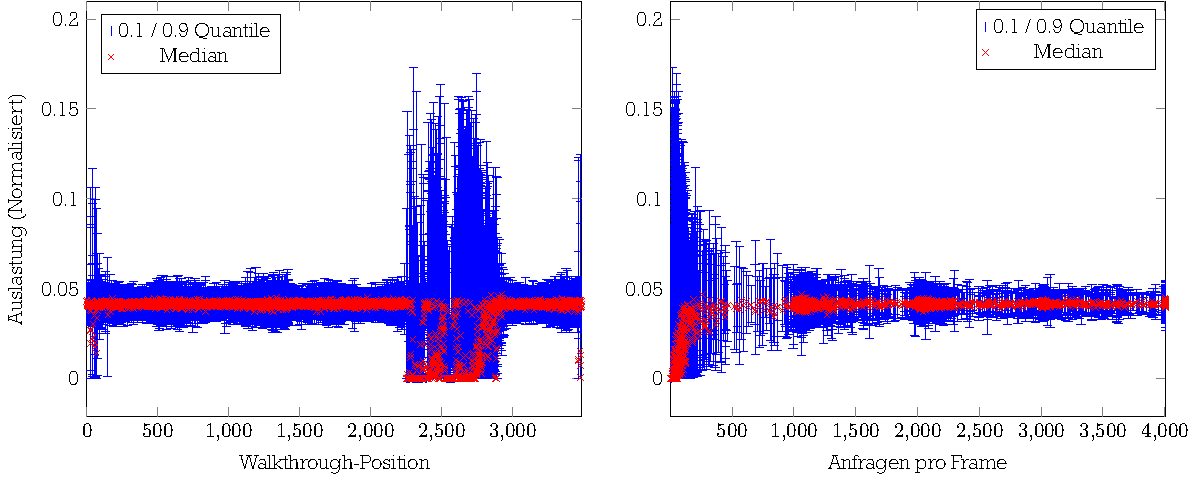
\includegraphics[scale=0.75]{images/diag_cCol_red1_render4_data24_2x.pdf}
  \captionof{figure}{\label{fig:eval:cCol1}Die Auslastung der Datenknoten in einem Walkthrough bei 4 Renderknoten und 24 Datenknoten und Redundanz$=$1.}
\end{Bild}

\begin{Bild}
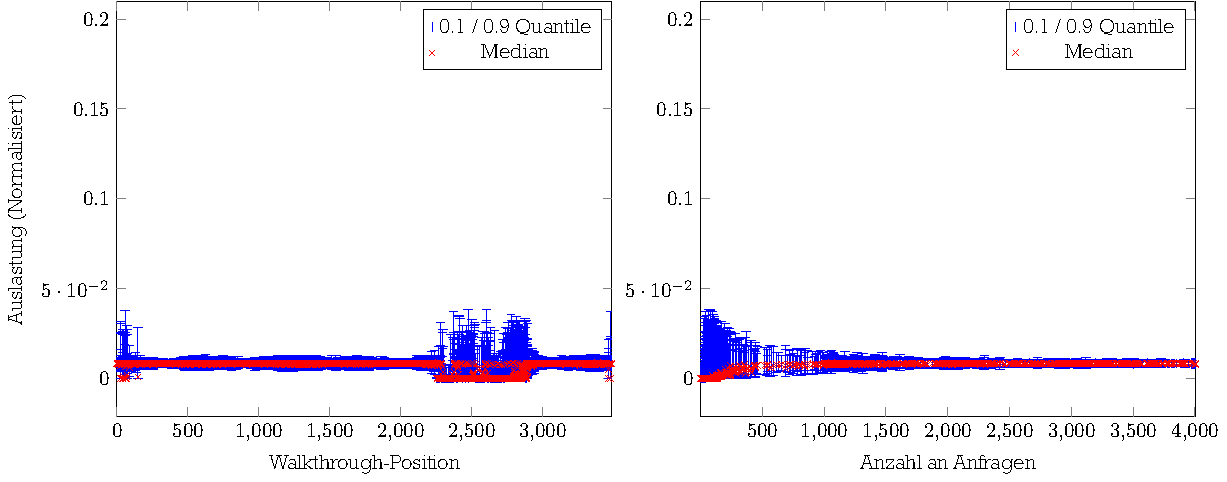
\includegraphics[scale=0.75]{images/diag_cCol_red3_render4_data120_2x.pdf}
  \captionof{figure}{\label{fig:eval:cCol9}Die Auslastung der Datenknoten in einem Walkthrough bei 4 Renderknoten und 120 Datenknoten und Redundanz$=$3.}
\end{Bild}
